\documentclass[00_complete]{subfiles}

\title{Mathematical Methods}
\author{Moshe Krumbein}
\date{Fall 2021}

\begin{document}
\Chapter{Coordinate Systems and Simple Geometric Shapes}{2}

\section{Circle}

Equation: $x^2+y^2=1$

Parametric: $\binom{\cos t}{\sin t}_{0 \leq t \leq 2 \pi}$

Two operations on shapes:
\begin{enumerate} \tightlist
    \item Transformation by a vector $\binom{a}{b}$
    \item Stretching by $c$ width-wise, $d$ height-wise
\end{enumerate}

Given parameterization $\binom{x(t)}{y(t)}$ or an equation $T(x,y)$:

Transformation by a vector $\binom{a}{b}$:
$$\binom{x(t) + a}{y(t) + b} \quad T(x-a, y-b)$$

Stretching by $c$ width-wise, $d$ height-wise:
$$\binom{c \cdot x(t)}{d \cdot y(t)} \quad T\left(\frac{x}{c}, \frac{y}{d}\right)$$

\section{Hyperbola}
We start from the following equation:
$$xy=c \implies y=\frac{c}{x}$$

Let's rotate this function $45 \degree$ counter-clockwise:

\begin{figure}[ht]
    \centering
      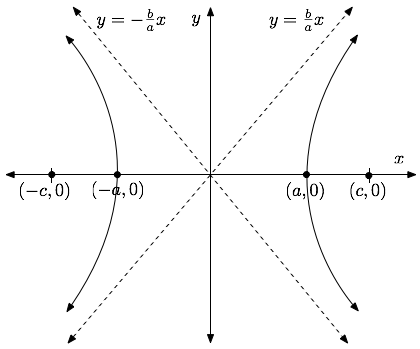
\includegraphics[width=0.5\textwidth]{hyperbola}
\end{figure}

To define our new function, we now define ${u,v}$ on the plane in how they
relate to our initial $(x,y)$.

We can do this by using projections of $x$ and $y$ onto our new $u, x$ axes:
$$
\begin{gathered}
    u = (x,y) \cdot \underbrace{\left( \frac{1}{\sqrt 2}, \frac{1}{\sqrt 2}\right)}_{\text{Unit vector of $u$}} = \frac{1}{\sqrt 2}( x+y) \\
    u = (x,y) \cdot \underbrace{\left(-\frac{1}{\sqrt 2}, \frac{1}{\sqrt 2}\right)}_{\text{Unit vector of $v$}} = \frac{1}{\sqrt 2}(-x+y)
\end{gathered}
$$

\begin{conclusion}
$$
\begin{gathered}
    uv = \alpha \\
    y^2 - x^2 = \frac{\alpha}{2} \\
    x^2 - y^2 = c \iff uv = -\frac{c}{2}
\end{gathered}
$$
\end{conclusion}

After stretching by $a$ in the direction of the $x$-axis and by $b$ in the
direction of the $y$-axis:
$$\frac{x^2}{a^2} - \frac{y^2}{b^2} = c$$

With the new asymptotes being:
$$y=\pm x \implies y=\pm x \cdot \frac{b}{a}$$

\section{Polar Coordinates}

Besides for the \emph{Cartesian} coordinate system (which is defined by how far a
point is from the $x$ and $y$-axis), we have the \emph{polar} coordinate system,
which is defined by the distance between the point and the origin (radius $r$) and
the angle between the $x$-axis and the point (angle, $\theta$).

Converting between representations:
$$
\begin{gathered}
  x \to r \cos \theta \quad y \to r \sin \theta \\
  r = \sqrt{x^2+y^2} \quad \theta = \tan^{-1}\left(\frac{y}{x}\right)\underbrace{(+ \pi)}_{\text{If $x<0$}} +2 \pi k
\end{gathered}
$$

A circle shifted by $a$ to horizontally with a radius of $a$:

$$
\begin{gathered}
    (x-a)^2+y^2=a^2 \\
    r = 2a \cos \theta
\end{gathered}
$$

\section{Cylindrical Coordinates}

The \emph{cylindrical coordinate system} is essentially the polar system just with a
third dimension $z$, where the radius is the distance from the $z$-axis (rho,
$\rho$), the angle ($\theta$), and z ($z$), such that:

$$x = \rho \cos \theta \quad y = \rho \sin \theta \quad z = z$$

\section{Solid of Revolution}

A \emph{solid of revolution} is made by taking a line (such as parabola) and rotating
around in the three dimensions to make a three-dimensional solid (in the case of
starting with a parabola, we create a \emph{paraboloid}).

Suppose a shape that is defined by $z=f(x)$. To rotate around the $z$-axis:

$$
\begin{gathered}
    \rho=\sqrt{x^2+y^2} \\
    z=f\left(\sqrt{x^2+y^2}\right)
\end{gathered}
$$

Parameterially:

$$z=f(x) = \begin{pmatrix}
    t \\ \square \\ f(t)
\end{pmatrix}
\quad
z=f\left(\sqrt{x^2+y^2}\right) = \begin{pmatrix}
    t \cos \theta \\ t \sin \theta \\ f(t)
\end{pmatrix}$$

\begin{example}
$$
\begin{gathered}
    z^2-y^2-y^2=4 \implies z^2 - (\overbrace{x^2+y^2}^{\rho^2})=4
\end{gathered}
$$

\begin{figure}[ht]
    \centering
      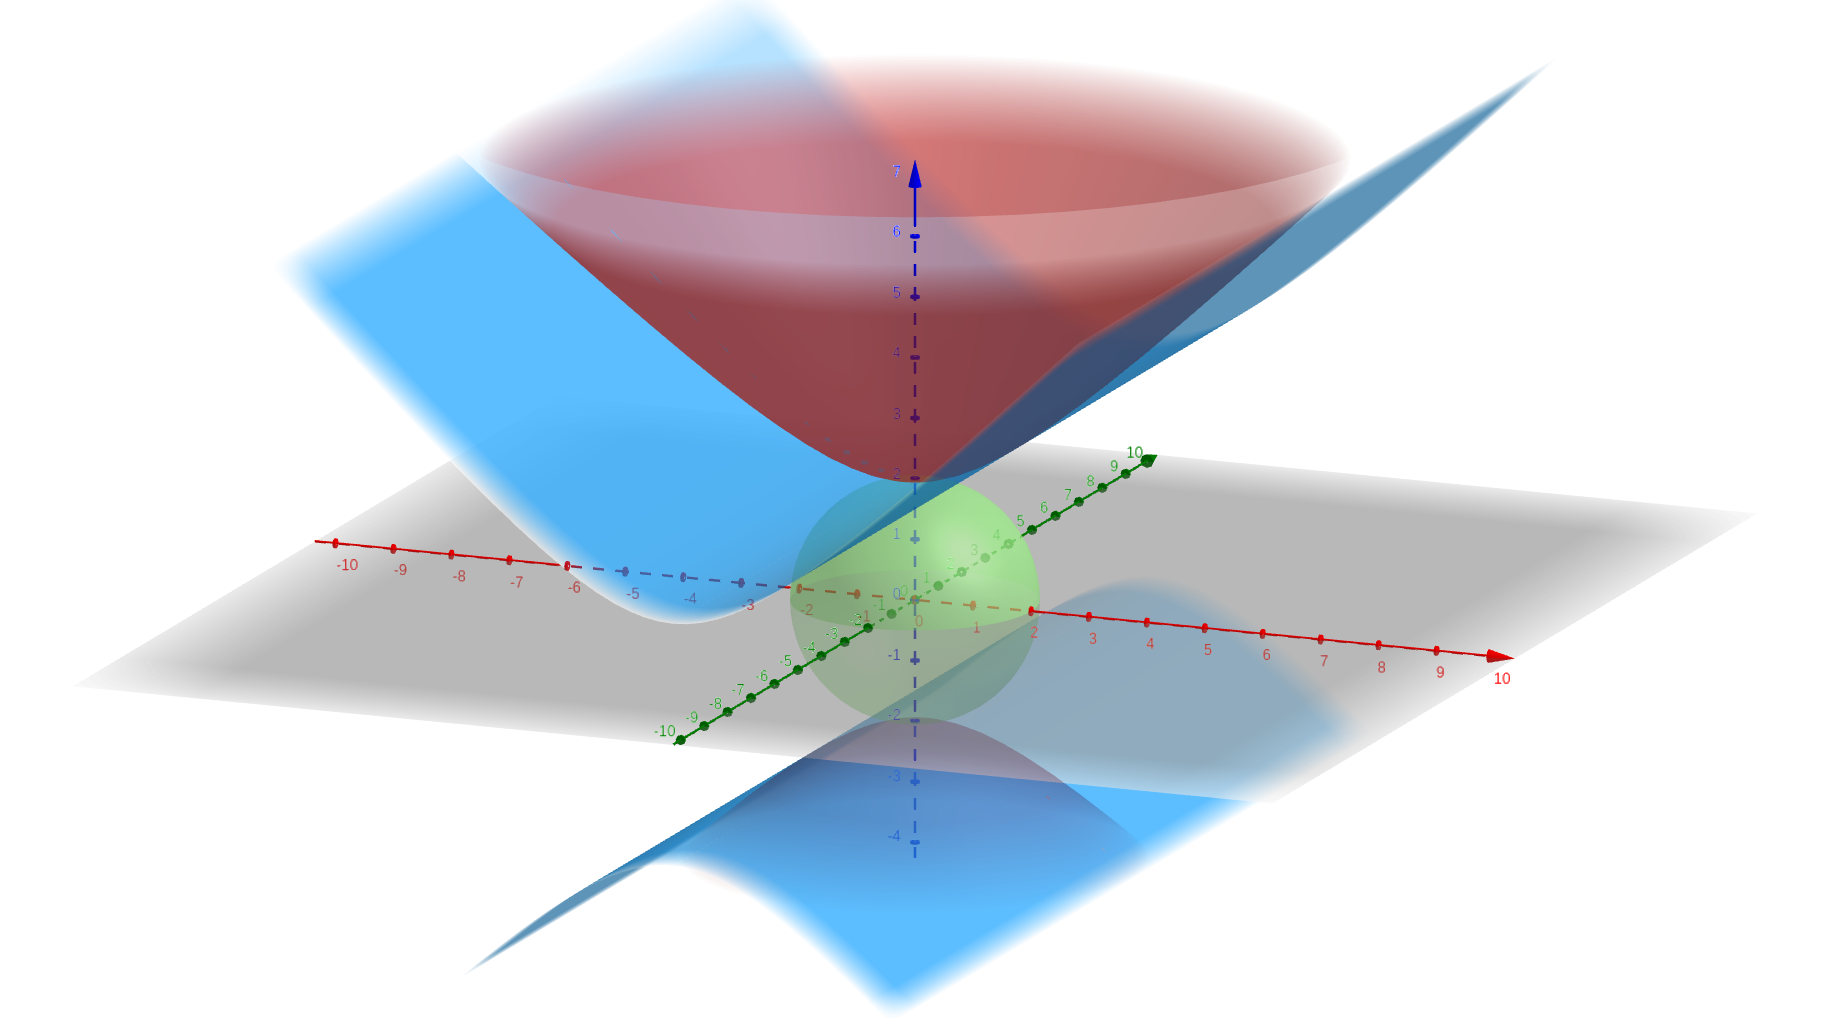
\includegraphics[width=0.5\textwidth]{fig2}
$$
\begin{gathered}
    \text{Red: } z^2-y^2-x^2=4 \\
    \text{Blue: } z^2-x^2=4 \\
    \text{Green: } z^2+y^2+x^2=4 \\
\end{gathered}
$$
\end{figure}

We have three points on a plane:

$$A=(1,2,3) \quad B=(1,1,1) \quad C=(6,-4,0)$$

To express the plane parametrically, we take two vectors from our points (such
as $\vec{AB}, \vec{BC}$)

$$
\begin{gathered}
    \vec{AB} = B - A = \begin{pmatrix}
        0\\-1\\-2
    \end{pmatrix} \\
    \vec{BC}  =C - B = \begin{pmatrix}
        5\\-5\\-1
    \end{pmatrix} \\
    \left\{\begin{pmatrix}
        1\\2\\3
    \end{pmatrix} + s \begin{pmatrix}
        0\\-1\\-2
    \end{pmatrix} + t \begin{pmatrix}
        5\\-5\\1
    \end{pmatrix} \mid s,t \in \mathbb{R}\right\}
\end{gathered}
$$

\end{example}

\section{Parameterization of Hyperbolae}
$$
\begin{gathered}
    x^2=y^2= c \\
    \begin{cases}
        x+y = t \\
        x-y = \frac{c}{t}
    \end{cases} \\
    x=\frac{1}{2}\left(t+\frac{c}{t}\right) \\
    y=\frac{1}{2}\left(t-\frac{c}{t}\right) \\
\end{gathered}
$$

$$\begin{gathered}
    x^2-y^2=-1:
    \begin{pmatrix}
        \frac{1}{2}\left(t-\frac{1}{t}\right) \\
        \frac{1}{2}\left(t+\frac{1}{t}\right) \\
    \end{pmatrix}
\end{gathered} \quad \vline \quad
\begin{gathered}
    (x+1)^2-\left(\frac{y+1}{\sqrt{\frac{1}{2}}}\right)=-1: \\
    \begin{pmatrix}
        \frac{1}{2}\left(t-\frac{1}{t}\right)-1 \\
        \frac{1}{2\sqrt 2}\left(t+\frac{1}{t}\right)-1 \\
    \end{pmatrix}
\end{gathered}$$

$y=x^2$ to rotate around the $x$-axis:

$$
\begin{gathered}
    y \mapsto \pm \sqrt{y^2+z^2} \\
    x^2 = \sqrt{y^2+z^2} \\
    x^4 = y^2+z^2 \\
\end{gathered}
$$

Parametrically:

$$\begin{pmatrix}
    t \\ t^2 \cos \theta \\ t^2 \sin \theta
\end{pmatrix}$$

\section{Spherical Coordinate System}

It consists of of the radius \(r\) (the distance of the point from the
origin), \(\theta\) (the angle above the \(x\)-axis towards the
\(y\)-axis), and \(\phi\) (the angle above the \(z\)-axis along
towards the point), such that:

\[
0 \leq \theta \leq 2 \pi \quad 0 \leq \phi \leq \pi
\]

In Cartesian coordinates: \[
\begin{gathered}
    x = r \sin \phi \cos \theta \\
    y = r \sin \phi \sin \theta \\
    z = r \cos \phi \\
    \\
    r = \sqrt{x^2+y^2+z^2} \\
    \phi = \cos^{-1}\left(\frac{z}{r}\right) \\
    \theta = \tan^{-1}\left(\frac{y}{x}\right) \underbrace{+\pi}_{y<0}
    = \cos^{-1}\left(\frac{x}{\sqrt{x^2+y^2}}\right)
    = \sin^{-1}\left(\frac{y}{\sqrt{x^2+y^2}}\right)
\end{gathered}
\]

\end{document}
